\documentclass[twoside, openright, 12pt]{book}
\sloppy

% Preamble
% General Setup
\usepackage{ifthen}		% If-Then-Statements
\usepackage{pdfpages}
\usepackage{hyperref}		% Hyperlinks & PDF specific information
\hypersetup{
	pdftitle={Master thesis - Philipp Schwetschenau},
	pdfsubject={Master thesis},
	pdfauthor={Philipp Schwetschenau},
	pdfborder={0 0 0}
}
\usepackage[nounderscore]{syntax}

% Language & Encoding
\usepackage[T1]{fontenc}
\usepackage[USenglish]{babel}
\usepackage[fixlanguage]{babelbib}
\usepackage[utf8]{inputenc}
\usepackage{blindtext}
\usepackage{caption}

% Page Geometry
\usepackage[a4paper]{geometry}
\geometry{
	twoside,
	top=3cm,
	bottom=3cm
}

% Literature
\usepackage{url}
\usepackage[sort&compress,square,comma,authoryear]{natbib}

% Fonts & Symbols
\usepackage{latexsym}		% Rare symbols
\usepackage{amsfonts}		% Math fonts
\usepackage{amssymb}		% Symbols
\usepackage{amsmath}		% Symbols
\usepackage{lmodern}		% "Latin Modern" ("Computer Modern"++)

\newcommand{\origttfamily}{}	% Separator for typewriter
\let\origttfamily=\ttfamily
\renewcommand{\ttfamily}{\origttfamily \hyphenchar\font=`\-}


%
% Document Layout

\usepackage[activate]{pdfcprot}	% margin kerning

% Header & Footer
\usepackage{fancyhdr}		% format headers
\pagestyle{fancy}
\fancyhf{}
\setlength{\headheight}{15pt}
\fancyhead[LE,RO]{\sffamily \thepage}
\fancyhead[RE]{\sffamily \nouppercase{\leftmark}}
\fancyhead[LO]{\sffamily \nouppercase{\rightmark}}
\renewcommand{\headrulewidth}{0.4pt}
\fancypagestyle{plain}{
	\fancyhead[RE,LO]{}
	\renewcommand{\headrulewidth}{0pt}
}
\fancypagestyle{simple}{
	\fancyhead[RE,LO]{}
	\renewcommand{\headrulewidth}{0pt}
}
\fancypagestyle{light}{
	\fancyhead[RE,LO]{}
}

% ClearDoublePage fix
\makeatletter 
\def\cleardoublepage{\clearpage\if@twoside \ifodd\c@page\else% 
\hbox{}% 
\thispagestyle{simple}
\newpage% 
\if@twocolumn\hbox{}\newpage\fi\fi\fi}
\makeatother 

% Headlines
\usepackage{titlesec}
\setcounter{secnumdepth}{3}
\titleformat{\chapter}[display]%
	{\huge\center\bf}%
	{\large\mdseries CHAPTER \thechapter}%
	{0cm}{}[\vspace{2ex}\titlerule]
\titlespacing*{\chapter}{0pt}{0ex}{8ex}
\titleformat{\subsubsection}{\normalsize\bfseries}{\thesubsubsection}{.75em}{}
\titleformat{\paragraph}[runin]{\bfseries}{}{0pt}{}[.]
\titleformat{\subparagraph}[runin]{\itshape}{}{0pt}{}[.]

% Table of Contents
\usepackage[titles]{tocloft}

\setlength{\cftbeforetoctitleskip}{0ex}
\setlength{\cftaftertoctitleskip}{0ex}
\renewcommand{\cfttoctitlefont}{}

\setlength{\cftbeforeloftitleskip}{4ex}
\setlength{\cftafterloftitleskip}{1ex}
\renewcommand{\cftloftitlefont}{\LARGE}

\setlength{\cftbeforelottitleskip}{4ex}
\setlength{\cftafterlottitleskip}{1ex}
\renewcommand{\cftlottitlefont}{\LARGE}

\newcommand\listingname{Verzeichnis der Listings}
\newlistof[chapter]{listing}{lst}{\listingname}
\setlength{\cftbeforelsttitleskip}{4ex}
\setlength{\cftafterlsttitleskip}{1ex}
\renewcommand{\cftlsttitlefont}{\LARGE}

\newcommand\theoremsname{Theoremverzeichnis}
\newlistof[chapter]{theorems}{lthm}{\theoremsname}
\setlength{\cftbeforelthmtitleskip}{4ex}
\setlength{\cftafterlthmtitleskip}{1ex}
\renewcommand{\cftlthmtitlefont}{\LARGE}

\setcounter{tocdepth}{2}
\setlength{\cftbeforechapskip}{1.0ex}
\setlength{\cftbeforesecskip}{0ex}
\setlength{\cftbeforesubsecskip}{-.2ex}
\newcommand\tocentry[1]{\addcontentsline{toc}{chapter}{#1}}
\newcommand{\ttsubsection}[1]{\subsection[\texorpdfstring{\texttt{\slshape #1}}{#1}]{\texttt{#1}}}
\newcommand\addtotheorems[2]{
	\refstepcounter{theorems}
	\addcontentsline{lthm}{theorems}{\protect\numberline{\thetheorems}\textbf{#1:} #2}
}
\newcommand\addlistspace[1]{
	\addtocontents{#1}{\vspace{1.3ex}}
}

% Glossar
\usepackage[number=none,style=altlist]{glossary}
\renewcommand{\glosslabel}[2]{\sffamily #2}
\makeglossary


%
% Page Elements

% Captions & Figures
\usepackage{graphicx}		% include graphics
\graphicspath{{./figures/}}

% Tables
\usepackage{booktabs}

% Theorems
\usepackage{framed}		% Frames for theorems.
\usepackage[framed,thmmarks,amsmath]{ntheorem}	% extended theorem enviroments
\usepackage{shadethm}		% theorems with colored background
\theoremheaderfont{\sffamily\bfseries}
\theorembodyfont{}
\theoremstyle{break}
\theoremseparator{.}
\theoremindent0cm
\theoremsymbol{}

\newshadetheorem{xtheorem}{Theorem}[chapter]
\newshadetheorem{xlemma}[xtheorem]{Lemma}
\newshadetheorem{xdefinition}[xtheorem]{Definition}
\newshadetheorem{xrequirement}[xtheorem]{Requirement}

\newenvironment{theorem}[1][]{%
	\addtotheorems{Theorem}{#1}
	\begin{xtheorem}[#1]%
}{\end{xtheorem}}
\newenvironment{lemma}[1][]{%
	\addtotheorems{Lemma}{#1}
	\begin{xlemma}[#1]%
}{\end{xlemma}}
\newenvironment{definition}[1][]{%
	\addtotheorems{Definition}{#1}
	\begin{xdefinition}[#1]%
}{\end{xdefinition}}
\newenvironment{requirement}[1][]{%
	\addtotheorems{Requirement}{#1}
	\begin{xrequirement}[#1]%
}{\end{xrequirement}}

\newshadetheorem{xapxtheorem}{Theorem}[section]
\newenvironment{apxtheorem}[1][]{%
	\addtotheorems{Theorem}{#1}
	\begin{xapxtheorem}[#1]%
}{\end{xapxtheorem}}

\theoremstyle{nonumberplain}
\theoremseparator{.}
\theoremheaderfont{\sffamily\itshape}
\theoremsymbol{\ensuremath{\Box}}
\newtheorem{proof}{Proof}
\newtheorem{apxproof}{Proof}

% Listings
\usepackage{listings}
\lstset{
	basewidth={0.5em,0.45em},
	frame=lines,
	framerule=\lightrulewidth,
	captionpos=b,
	lineskip=-1pt,
%	float=hbt,
	xleftmargin=1cm,
	xrightmargin=1cm,
	aboveskip=0.5cm,
	belowskip=0.5cm,
}
\lstnewenvironment{java}[2]{
	\refstepcounter{listing}
	\addcontentsline{lst}{listing}{\protect\numberline{\thelisting}#1}
	\lstset{
		language=C++,
		basicstyle=\ttfamily,
		commentstyle=\sffamily,
		lineskip=-2pt,
		tabsize=4,
		#2
	}
}{}
\lstdefinelanguage{pseudocode}{
	sensitive=true,
	alsodigit={:},
	morekeywords={
		Algorithmus,Eingabe:,Ausgabe:,Variablen:,%
		when,if,then,else,end,atomic,out,%
		case,is,repeat,while,do,until},
}
\lstdefinelanguage[distributed]{pseudocode}
	[]{pseudocode}{
	alsodigit={:},
	morekeywords={Async,Sync,%
		Constants:,Variables:,Input:,Action:,Action,%
		send,to,from},
	deletekeywords={Algorithmus,Eingabe:,Ausgabe:,Variablen:}
}
\newcommand{\setpseudocode}[2]{
	\lstset{
		% Syntax
		language=[#1]{pseudocode},
		mathescape=true,
		escapechar=\#,
		tabsize=4,
%		gobble=4,
		literate={:=}{{$\gets$}{\:}}2 {->}{{$\rightarrow$}{\:}}2,
		% Style
		basicstyle=\rmfamily,
		commentstyle=\sffamily,
		moredelim=[is][\itshape]{//}{//},
		moredelim=[il][\sffamily]{**},
		% Layout & Placement
		numbers=left,
		numberstyle=\tiny,
		columns=flexible,
		breaklines=true,
		breakatwhitespace=true,
		breakindent=2em,
		% User defined
		#2
	}
}
\lstnewenvironment{distalg}[2]{%
	\refstepcounter{listing}
	\addcontentsline{lst}{listing}{\protect\numberline{\thelisting}#1}
	\setpseudocode{distributed}{#2}
}{}
\lstnewenvironment{pseudocode}[2]{%
	\refstepcounter{listing}
	\addcontentsline{lst}{listing}{\protect\numberline{\thelisting}#1}
	\setpseudocode{}{#2}
}{}

\newcommand\textcall[1]{\textsc{#1}}
\newcommand\call[2]{\ensuremath{\operatorname{\textcall{#1}}(#2)}}
\newcommand\callname[2]{\ensuremath{\operatorname{#1}(#2)}}
\newcommand\topin[1]{\ensuremath{\operatorname{In}({#1})}}
\newcommand\topout[1]{\ensuremath{\operatorname{Out}({#1})}}


%
% Inline
\usepackage{url}		% Cite URLs
\usepackage{numprint}		% Format numbers
\newcommand\notice[1]{}		% Notice
\newcommand\seppar{ \vspace{2ex} \noindent } % New paragraph
\newcommand\name[1]{{\em #1}} 	% Names


\newenvironment{BNF}
  {\captionsetup{type=lstlisting}}
  {}

\begin{document}

%
% Titelseite
\begin{titlepage}
\newlength{\detailwidth}
\newlength{\detaildescriptionwidth}
\settowidth{\detailwidth}{Eingereicht:~~ Prof. Dr.-Ing. habil. Winfried E. Kühnhauser}
\settowidth{\detaildescriptionwidth}{Studies:~~} 
\begin{center}

\vfill {
	
\includegraphics[width=6cm]{logo-tu-ilmenau.jpg}
	\vspace{8ex}
}

\begin{normalsize}Technische Universität Ilmenau \\
Fakultät für Informatik und Automatisierung \\
Institut für Praktische Informatik und Medieninformatik \\
Fachgebiet für Verteilte Systeme und Betriebssysteme        
\end{normalsize}


\vfill {\large
	Master's thesis\\ \vspace{2ex}
	\LARGE \textbf{Graphical Specification Language \\for the Entity-Labeling Aspect} \\ \vspace{2.5ex} 
	\normalsize Submitted by: \\
	\Large Philipp Schwetschenau \\ \vspace{3ex} 
}
\vfill \parbox{\detailwidth}{
	\makebox[\detaildescriptionwidth][r]{Supervisor:~~} Prof. Dr.-Ing. habil. Winfried E. Kühnhauser \\
	\makebox[\detaildescriptionwidth][r]{Supervisor:~~} Dipl.-Inf. Peter Amthor \\
	\vspace{2ex} \\
	\makebox[\detaildescriptionwidth][r]{Studies:~~} Computer science\\  
	\makebox[\detaildescriptionwidth][r]{Matriculation no.:~~} 46756  
	\vspace{2ex} \\
	\makebox[\detaildescriptionwidth][r]{Submission:~~} Ilmenau, 29. November 2018 (planned)
}
\vspace*{\fill}
\end{center}
\end{titlepage}

\mbox{}
\thispagestyle{empty}
\cleardoublepage

% Gliederung
\pagenumbering{roman}
\setcounter{page}{1}
\tableofcontents

% Abbildungsverzeichnis
\cleardoublepage
\listoffigures
\tocentry{List of figures}

%\listoflisting
%\tocentry{\listingname}

%
% Citing

% Author 1 et al. [1234]
%\cite{Harrison75a}

% Author 1, Author 2, Author 3 [1234]
%\cite*{Harrison75a}

% [Author 1 et al. 1234]
%\citep{Harrison75a}

% [Author 1, Author 2, Author 3 1234]
%\citep*{Harrison75a}



% Inhalts-Teil
\cleardoublepage
\pagenumbering{arabic}
\chapter{Introduction}
\label{introduction}

\section{Domain} 
\label{domain}
With the increasing number of IT systems, securing these systems became an obvious and important issue.
For this purpose many security models and model families were developed for a wide field of application domains over the last years.

Formal security models offer possibilities to analyze them concerning security properties.
However, because quantity and variety of these models grow just as much as their relevance for security-critical applications the model-based security engineering process became more complex and therefore error-prone to human deviations.

\citet*{Amthor18} proposed a new approach called Aspect-oriented Security Engineering (AOSE) which claims to close semantic gaps between steps in the security engineering process (requirements, informal policy, formal model) to reduce the potential impact of human errors.
This approach roughly adopts the idea of the aspect-oriented programming paradigm.
It tailors all steps to aspects, which are non-functional requirements of the engineering process like determining requirements of policy semantics or analyzing certain security goals.
There are two major classes for aspects regarding AOSE: related to policy semantics and to policy analysis.

One possible aspect of the former is the Entity Labeling Aspect (EL).
It is designed to formally specify policy semantics typically found in operating systems and middleware systems.
Therefore it bridges the gap and supports the transformation between informal policy and formal model.
EL classifies model components into six semantic categories.
The notation is on a mathematical basis and uses concepts like sets, assignments or constraints.



\section{Motivation} 
\label{motivation}
The goal of reducing the impact of human errors by closing semantic gaps as much as possible with the help of AOSE/EL requires handling another formal notation, which is, in this case, EL itself and its classification into the six semantic categories.
To support working with this approach, especially for the communication between different groups of people involved like model engineers, security architects, software developers or future administrators, who have to cooperate and coordinate and all have different levels of experience, \citet*{Amthor18} considers a graphical representation to be helpful to enhance the transition between informal and formalized notation.

\citet*{Amthor18} already uses visual representations to illustrate examples.
However, the representations are not described in detail as well as they are inconsistent and ambiguous regarding several parts of the formalization (e.g.\ arrows can have several meanings and there is no way to specify functions with multiple input parameters).
So these visualizations are appropriate to underline and support the engineering of an already formalized policy after EL-based model engineering, but are not suitable for independent modeling on a stand-alone level, because they are not equivalent to their formalized mathematical counterpart.

There are two types of visualization \cite{Amthor18} uses, which have different levels of abstraction: 
One is based on the actual model components and visualizes them and their relationships.
The other one is based on a higher level of abstraction and visualizes the EL with its structure of semantic categories and their relationships.

There are other visual notations like UML or ERD, which have in common that they are tailored to particular needs in special application domains, so they can not be applied here, but may give inspiration on how to model certain semantics and relationships.

Eventually to be able to independently and visually model and work on EL-based policies there is need for an unambiguous formal graphical specification language.



\section{Goal}
\label{goal}
The main goal is to develop a graphical specification language for EL-based security polices.
This should focus on clean and unambiguous semantics of the language.

The use of the language should be as simple as possible and as comprehensive as needed.
Therefore its appearance and elements should be clear and well-structured.
A selection of appropriate symbols and geometrical shapes for their equivalent model counterparts has to be made regarding an intuitive understanding and workflow.
This selection should not be designed contradictory or conflicting to already established notations, especially those, which may be used in the context of security engineering.

It should be evaluated how feasible and reasonable it is to develop equivalent counterparts for every possible element and relationship in context of EL and to display all of them at once.
This may also lead to the question how the visualization is related to a visualization on a higher abstraction level and how they are connected and might be managed.
The latter may be investigated as an optional goal.

In addition to that a GUI-based editor should be developed as a prototype to make use of the proposed graphical specification language.



\section{Structure}
\label{structure}




\cleardoublepage
\chapter{Fundamentals}
\label{fundamentals}
This chapter provides information to fundamentals necessary for this thesis.
It will serve as a basis for design decisions in the following chapter~\ref{gsl_design} and chapter~\ref{editor_design}.

Section \ref{security_models} introduces two fundamental families of security models: IBAC and RBAC.
It also describes a graphical notation for depicting RBAC models by \cite{Sandhu96}.
This notation will serve as first basis for graphical modeling in this domain.
Section \ref{AOSE} focuses on the Aspect-oriented Security Engineering (AOSE) proposed by \citet*{Amthor18}.
It covers the Entity Labeling Aspect in particular, one aspect of AOSE, which is going to be essential regarding the task to design a graphical specification language for it.
Also the notation used by \citet*{Amthor18} to graphically model the process of Entity-Labeling, which was inspired by the graphical RBAC notation by \cite{Sandhu96}, will be described.
This will be the starting point in designing the graphical specification language in chapter \ref{gsl_design}.

In section~\ref{graphical_notations} the well-established graphical notations \textit{Unified Modeling Language} and \textit{Entity-Relationship} are described.
Based on human optical perception and gestalt laws section~\ref{perception} provides information on how we perceive and evaluate optical stimuli regarding properties like shape and closeness.
In the last section~\ref{gui_design} information on how to design a software graphical user interface are given with respect to common best practices like interaction design patterns and usability.

\section{Security models}
\label{security_models}
A \textit{security policy} is a set of rules to fulfill security related requirements of an IT system.
In order to be able to work with such a security policy and to analyze it, it has to be formalized as an instance of a \textit{security model}.
Being the central artifact in the process of model-based security engineering we want to describe a very basic security model -- the \textit{Identity-based Access Control} (IBAC) model -- and a well-established and widely used extension of it -- the \textit{Role-based Access Control} (RBAC) model.
In the course of this work, we need security policies and models to explain and visualize model-based security engineering with regard to Entity Labeling.

%\subsection{HRU}
%\label{HRU}
%The HRU security model \citep*{Harrison75a} is a fundamental, dynamic access control model.
%It manages permissions of subjects on objects with the help of an state automaton and access control matrices.
%While subjects are active (e.g. users), objects are passive (e.g. files).

%\begin{xdefinition}[HRU] 
%A HRU model is a deterministic automaton
%$(Q, \Sigma , \delta , q_{0})$ with 
%$Q = 2^S \times 2^O \times M$ as state space, 
%$M = \lbrace m|m:S \times O \rightarrow 2^R \rbrace$ as set of access control matrices, 
%$\Sigma$ as input alphabet, 
%$\delta : Q \times \Sigma \rightarrow Q$ as state transition function and 
%$q_0 \in Q$ as initial state.
%\end{xdefinition}



\subsection{Identity-based Access Control}
\label{IBAC}
The most fundamental class of security models is probably the family of Identity-based Access Control (IBAC) models.
The model is based on a system with active (subjects) and passive entities (objects).
In IBAC requests are decided according to the unique identification of the requester and the object \citep{Lampson74}.
A set of rules (\textit{policy}) determines whether a request is permitted or forbidden.
These rules can be formulated as access control matrix (ACM) or access control function (ACF).
An ACF is defined as following \citep{Amthor18}:

\begin{definition}[Access control function]
An access control function (ACF) is a function ${acf}: S \times O \times OP \rightarrow \mathbb{B}$, where
\vspace{-2mm}
\begin{itemize}
\item $S$ is a set of \textit{subject identifiers}
\item $O$ is a set of \textit{object identifiers}
\item $OP$ is a set of \textit{operation identifiers}
\end{itemize} 
\vspace{-2mm}
For any $s \in S, o \in O, op \in OP$, we say $s$ is allowed to execute $op$ on $o$ iff $acf(s,o,op)$.
\end{definition}



\subsection{Role-based Access Control}
\label{RBAC}
With an increasing number of subjects and objects the access control functions/matrices of IBAC models get very large and hard to manage effectively.
Role-based Access Control (RBAC) models counter this scalability problem by adding one stage of indirection.
For this RBAC models extend IBAC with the concept of roles \citep{Sandhu96}.
This design decision is based on the finding of \cite{Sandhu96} that in large systems many subjects share the same access privileges.
On the one hand every user is mapped to a set of roles.
On the other hand every role is mapped to a set of permissions.
This concept reduces redundancy in systems with large or fast growing sets of subjects and objects and also models real scenarios closer to reality (e.g. job function in an organization).

\begin{xdefinition}[RBAC] 
A RBAC$_0$ model is a tuple $(U, R, P, S, UA, PA, user, roles)$ with

\vspace{-2mm}
\begin{itemize}
\setlength\itemsep{0em}
\item $U$ as set of \textit{users}
\item $R$ as set of \textit{roles}
\item $P = 2^{O \times OP}$ as set of \textit{permissions}
\vspace{-2mm}
\begin{itemize}
\item $O$ is the set of \textit{objects}
\item $OP$ the set of \textit{operations})
\end{itemize}
\vspace{-2mm}
\item $S$ as set of \textit{sessions}
\item $UA \subseteq U \times R$ as a many-to-many \textit{user-to-role assignment relation}
\item $PA \subseteq P \times R$ as a many-to-many \textit{permission-to-role assignment relation}
\item $user: S \rightarrow U$ as function, that maps every session to a single user
\item $roles: S \rightarrow 2^R$ as function, that maps every session to set of roles
\end{itemize}
\label{definition:RBAC}
\end{xdefinition}

\noindent
RBAC is called a family of security models, because there is a base model (RBAC$_0$) and three models that extend this base model with advanced concepts.
RBAC$_1$ extends RBAC$_0$ with a role hierarchy, because in reality it turned out that roles are often combinations of other already existing roles.
This reduces redundancy and improves RBAC's scaling behavior even further.
The role hierarchy is defined as partial order $RH \subseteq R \times R$.% on $R$. %(also written as $\geq$).

RBAC$_2$ extends RBAC$_0$ with a set of constraints $C$ to restrict values of the model components $UA, PA, user, role$ or $RH$ (e.g. ``\textit{forbid the activation of two certain roles at the same time}'').
Constraints are highly individual and specific to a certain application.
However, \cite{Sandhu96} mentions three main concepts for constraints, that seem to be used frequently and are therefore reasonable to implement: \textit{Mutually exclusive roles}, \textit{cardinality} and \textit{prerequisite roles}.

RBAC$_3$ combines the concepts of RBAC$_1$ and RBAC$_2$.

%In contrast to automaton-based security models (e.g.~HRU), RBAC is static.
%Due to not being dynamic a RBAC model can always just reflect a snapshot in time.
%A dynamic variant of RBAC was proposed by \cite{Schlegel13} and is called DRBAC.
%It combines the RBAC$_3$ model with a deterministic state automaton of the HRU model.

%\begin{xdefinition}[DRBAC] 
%A DRBAC model is a tuple 
%$(Q, \Sigma , \delta , q_{0}, OP, R, RH, C)$ with
%$Q = 2^U \times 2^O \times 2^P \times 2^S \times 2^{\mathit{PA}} \times %2^{\mathit{UA}} \times \mathit{USER} \times \mathit{ROLES}$ as state space, where $U, O, P, S, PA, UA, RH, C$ is defined just as in the RBAC$_3$ model, 
%$\mathit{USER} = \lbrace user|user: S \rightarrow U \rbrace$ as set of mappings that maps sessions to users, 
%$\mathit{ROLES} = \lbrace roles|roles: S \rightarrow 2^R \rbrace$ as set of mappings that maps sessions to roles, 
%$\Sigma = OP \times X$ as input alphabet, 
%$\delta : Q \times \Sigma \rightarrow Q$ as state transition function, 
%$q_0 \in Q$ as initial state and 
%$OP, R, RH, C$ as static component.
%\end{xdefinition}



\subsubsection{RBAC notation by Sandhu at al.}
\label{RBAC_notation}
\cite{Sandhu96} use a graphical notation in their work to visualize the RBAC model family with all its elements and relationships (see figure \ref{fig:Sandhu_notation}).
Due to RBAC being a well-established security model and also regarding its relevance in literature -- especially for its contribution to the standardized NIST RBAC model \citep{RBACNIST} -- we want to take a closer look at its graphical notation.
Unfortunatly \cite{Sandhu96} gives no details on how or why the notation is build up the way it is in his work.

\begin{figure}[htb]
	\centering
	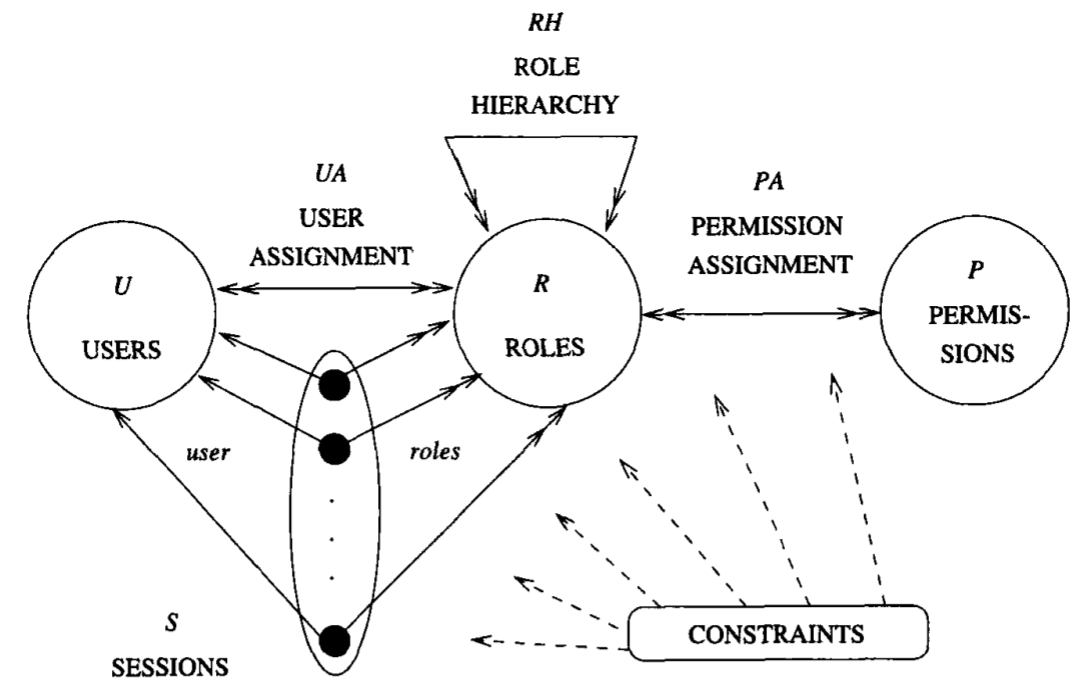
\includegraphics[width=\linewidth-2cm]{../figures/chapter2/Sandhu_notation.png}
	\caption{Graphical notation to visualize $RBAC_3$ by \cite{Sandhu96} }
	\label{fig:Sandhu_notation}
\end{figure}

\noindent
Following graphical elements are used in this notation:

\begin{itemize}
\item A circle or ellipse represents a set ($U, R, P, S$).
\item A rounded rectangle represents a special set -- the set of \textit{Constraints}.
\item A normal-headed unidirectional arrow represents a one-to-one assignment ($user$).
\item A double-headed unidirectional arrow represents a one-to-many assignment ($roles$).
\item A double-headed bidirectional arrow represents a many-to-many assignment relation ($UA, PA, RH$).
\item A normal-headed unidirectional dotted arrow represents a constraint.
Six arrows of this type are pointing symbolically from the set of constraints in the direction of all model components constraints can be potentially defined on.
\end{itemize}
%TODO: Better a table?

\noindent
A set has its name and its identifier in its center.
An arrow -- except the constraint arrow -- has its identifier and optionally its name next to it.

Furthermore the set \textit{Sessions S} is not directly connected with arrows to other components.
It is drawn with large black dots inside, which represent single elements of this set.
These set elements are then connected to other components with certain arrows.
Three small black dots (in this case aligned horizontally) indicate that those three set elements are just symbolic and that there are potentially more or less (the number of sessions is not limited per definition).

This diagram is often used in a simplified form (for example in \citep{Amthor18}) that does not display single set elements of \textit{Sessions S}, but directly connects \textit{Sessions S}-- like the other sets -- with just one arrow (for the \textit{user} function) to \textit{Users} and one arrow (for the \textit{roles} function) to \textit{Roles}.
Also worth mentioning is that the \textit{Role Hierarchy RH} is drawn as a loop. 
It is pointing from \textit{Roles} ($R$) to \textit{Roles} with a double-headed bidirectional arrow.

Sandhu's notation depicts the overall structure of the RBAC model with its relationships between model components.
Different arrow types indicate different types of relationships.
Besides \textit{Sessions S} no set displays any set elements.
Also no set displays any kind of definition for its elements.
For example \textit{Permissions P} does not indicate that its elements are defined as $2^{O \times OP}$ (as in the RBAC definition, see definition \ref{definition:RBAC}).

%maybe my own gsl from bachelor thesis?


%\subsection{Security Model Core}
%\label{model_core}
%Over the years many different security models emerged for special purposes and requirements.
%They heavily vary and differ in their structure and design.
%Comparing them or even parts of them for analysis or evaluation purposes is not always possible per se.
%Methods to analyze a model concerning a given security property have to be adapted to every model they should run on.
%So \cite{Poelck14} proposed the Security Model Core to describe and formalize all possible security models in one meta model in a homogeneous way.

%\begin{xdefinition}[Security Model Core]
%\label{def:SecurityModelCore}
%The Security Model Core is a 5-tuple 
%$(Q, \Sigma , \delta , q_{0}, E)$ with 
%$Q$ as state space,
%$\Sigma$ as input alphabet, 
%$\delta: Q \times \Sigma \rightarrow Q$ as state transition function, 
%$q_0$ as initial state and 
%$E$ as static extension vector.
%\end{xdefinition}

%The definition of model components depends on the specialization of the corresponding model core and is done in six steps by identifying and defining those components.



\section{Aspect-oriented Security Engineering}
\label{AOSE}
In this section the Aspect-oriented Security Engineering proposed by \cite{Amthor18} is described with focus on its Entity Labeling aspect.
The content of this section will act as fundamental basis of information for designing a graphical specification language for the Entity-Labeling aspect later in chapter \ref{gsl_design}.

Aspect-oriented Security Engineering (AOSE) is a new approach proposed by \cite{Amthor18} to improve the process of model-based security engineering.
With an increasing number and complexity of security models the engineering process that goes along also became more complex and therefore prone to human errors.
\cite{Amthor18} claims to close semantic gaps between model engineering, model analysis and formal policy specification in the process of security engineering to reduce the potential impact of human errors.
These three steps and how they connect are depicted in figure \ref{fig:AOSE}.

\begin{figure}[htb]
	\centering
	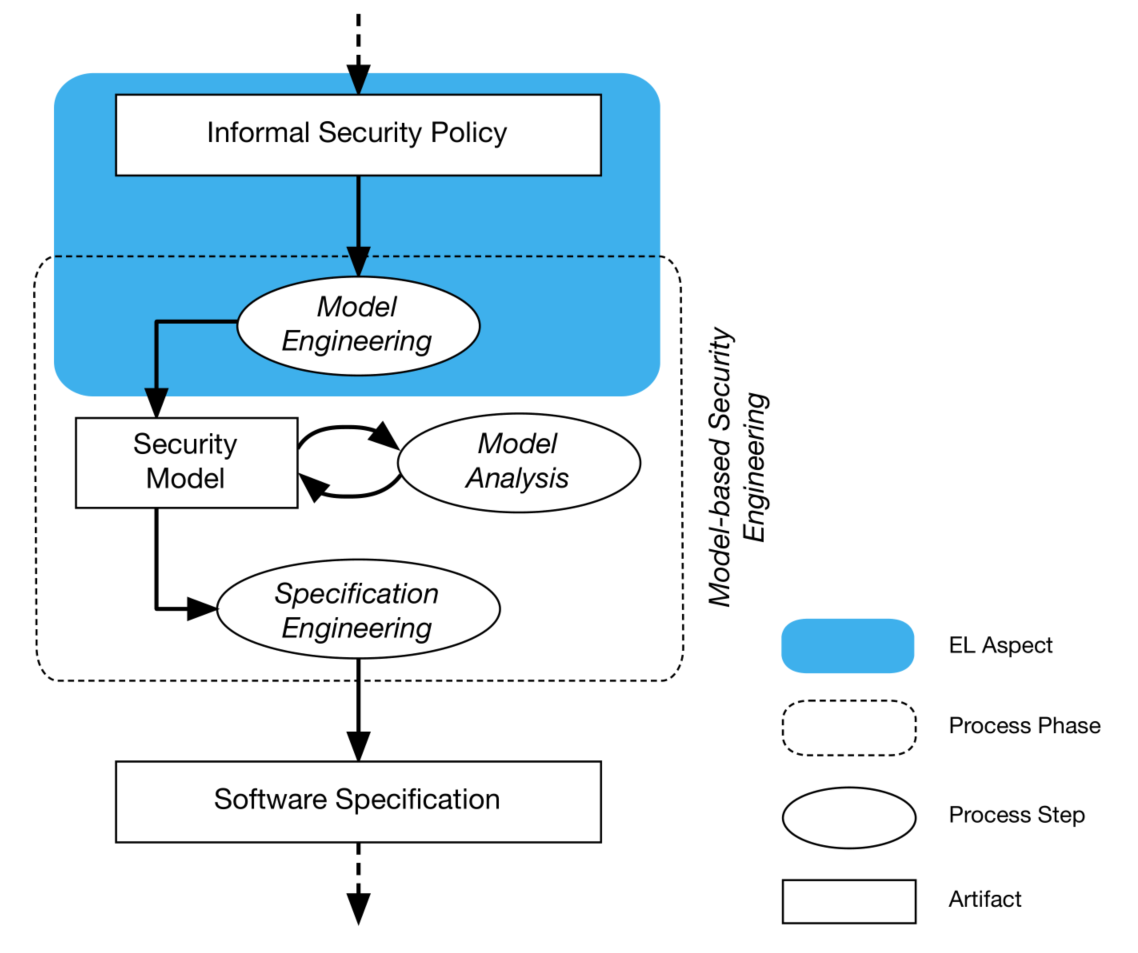
\includegraphics[scale=0.4]{../figures/chapter2/AOSE.png}
	\caption{Steps of model-based security engineering \citep{Amthor18}}
	\label{fig:AOSE}
\end{figure}

\noindent
AOSE roughly adopts the idea of the aspect-oriented programming paradigm.
It tailors all steps to aspects, which are non-functional requirements of the engineering process, for example determining requirements of policy semantics or analyzing certain security goals.
There are two major classes \cite{Amthor18} proposes for aspects regarding AOSE: related to policy semantics and related to policy analysis.
One of several aspects proposed in his work is Entity Labeling.

According to \cite{Amthor18} an aspect-oriented security model is defined as:

\begin{xdefinition}[Aspect-oriented security model] 
A aspect oriented security model is defined as 
\begin{gather*}
\langle \mathcal{M},\mathcal{A},sem \rangle
\end{gather*}
with:

\vspace{-2mm}
\begin{itemize}
\setlength\itemsep{0em}
\item $\mathcal{M}$ as finite set of model component identifiers
\item $\mathcal{A}$ as set of semantic category identifiers (aspect)
\item $sem : \mathcal{A} \rightarrow 2^\mathcal{M}$ as semantical application of $\mathcal{A}$ to $\mathcal{M}$
\end{itemize}
\label{definition:AOSE}
\end{xdefinition}



\subsection{Entity Labeling}
\label{EL}
The Entity Labeling (EL) aspect is one possible aspect $\mathcal{A}$ in context of AOSE (see definition \ref{definition:AOSE}).
It is designed to support the process of formally specifying policy semantics typically found in operating systems and middleware systems.
According to \cite{Amthor18} it bridges the gap between informal policy and formal model by supporting its transformation (see highlighted part in figure \ref{fig:AOSE}).

For this model components of an informally specified policy have to be identified and formalized by classifying them into the six semantic categories $ES$, $LS$, $LA$, $AR$, $RR$, and $MC$:

\begin{description}
\item[1) Entity Set (ES)]\hfill \\
\textit{ES} is a set of entity identifiers.
Basic elements in context of access control decisions are defined as \textit{entities} and are resources and principals like subjects or objects.
%\vspace{-2mm}

%\begin{xdefinition}[ES] 
%ES model components are sets that list potential participants in access decisions.
%Elements of those sets are (1) atomic identifiers, (2) legal argument values for any authorization decision, (3) illegal argument values for evaluating \textit{AR} model components and (4) associated with labels via \textit{LA} model components.
%\label{definition:ES}
%\end{xdefinition}

\item[2) Label Set (LS)]\hfill \\
\textit{LS} is a set of legal label values.
Labels act as attributes in access control decisions and therefore as level of indirection.
Their content vary depending on a policy's application domain and can be finite enumerations (e.g.~RBAC), infinite enumerations (e.g.~ABAC) or any number system such as $\mathbb{N}$.
%\vspace{-2mm}

%\begin{xdefinition}[LS] 
%LS model components are sets that list identifiers used in entity labels.
%Elements of those sets are (1) legal attribute values in labels, (2) legal argument values for evaluating \textit{AR} model components, (3) illegal argument values for any authorization decision and (4) may be associated with labels via \textit{LA} model components.
%\label{definition:LS}
%\end{xdefinition}

\item[3) Label Assignment (LA)]\hfill \\
\textit{LA} is a set of associations between entities and labels.
%\vspace{-2mm}

%\begin{xdefinition}[LA] 
%LA model components are assignments that determine a system configuration in terms of how a policy's access rules (\textit{AR}) are applied to entities (\textit{ES}). They (1) are used to associate entity identifiers with label identifiers, (2) may be used to associate label identifiers with label identifiers and (3) indirectly determine any authorization decision.
%\label{definition:LA}
%\end{xdefinition}

\item[4) Access Rule (AR)]\hfill \\
\textit{AR} is a logical rule that defines, based on a set of entity labels, which operations may be legally performed on entities corresponding to these labels. Model components in \textit{AR} thus reflect a policy’s access control function.
%\vspace{-2mm}

%\begin{xdefinition}[AR] 
%\textit{AR} model components are logical rules which (1) are evaluated using label identifiers and (2) directly determine any authorization decision.
%\label{definition:AR}
%\end{xdefinition}

\item[5) Relabeling Rule (RR)]\hfill \\
\textit{RR} is a logical rule for legal label changes.
Label changes can emerge from either administrative accesses (e.g.~RBAC's \textit{UA}) or discretionary accesses (user owns files and grant roles/users access).
%\vspace{-2mm}

%\begin{xdefinition}[RR] 
%\textit{RR} model components are logical rules which (1) define relations between \textit{ES} or \textit{LS} model components and (2) restrict changes of \textit{LA} model components.
%\label{definition:RR}
%\end{xdefinition}

\item[6) Model Constraints (MC)]\hfill \\
\textit{MC} is a set of constraints over model components that must be satisfied at all time.
There are two types of constraints: policy-intrinsic (related to variables managed inside the AC system) and policy-extrinsic (related to external variables, e.g.~time).
%\vspace{-2mm}

%\begin{xdefinition}[MC] 
%MC model components are boolean expressions or external variables. 
%They represent conditions which (1) may relate to all model components (including external variables), (2) must be satisfied by the values of all model components (excluding external variables) and (3) must be satisfied after any change of the model components.
%\label{definition:MC}
%\end{xdefinition}
\end{description}

%\noindent
%According to these categories EL is defined as following:

%\begin{xdefinition}[Entity Labeling aspect] 
%The Entity Labeling aspect of a security policy is defined as:
%\begin{gather*}
%\mathcal{A}_{EL} = \lbrace ES,LS,LA,AR,RR,MC\rbrace
%\end{gather*}
%where $ES$, $LS$, $LA$, $AR$, $RR$, and $MC$ denote categories of model components defined as in definitions \ref{definition:ES} to
%\label{definition:EL} \ref{definition:MC}.
%\end{xdefinition}

\noindent
The resulting model after EL can be depicted in three different forms: Textual, table and graphical.
The textual form created from an example policy looks like this:

\begin{align*}
\langle &\mathcal{M}_{example}, \mathcal{A}_{EL}, sem \rangle
\end{align*}
\begin{align*}
\mathcal{M}_{example} &= \lbrace U, D, R, GR, AR, P, ua, da, pa \rbrace
\end{align*}
\begin{align*}
sem(ES) &= \lbrace U, D \rbrace\\
sem(LS) &= \lbrace R, P \rbrace\\
sem(LA) &= \lbrace ua, da \rbrace\\
sem(AR) &= \lbrace pa, P \rbrace\\
sem(RR) &= \lbrace GR, AR, ua \rbrace\\
sem(MC) &= \lbrace \emptyset \rbrace
\end{align*}

\noindent
Figure \ref{fig:EL_table} shows the same result as table.

\begin{figure}[htb]
	\centering
	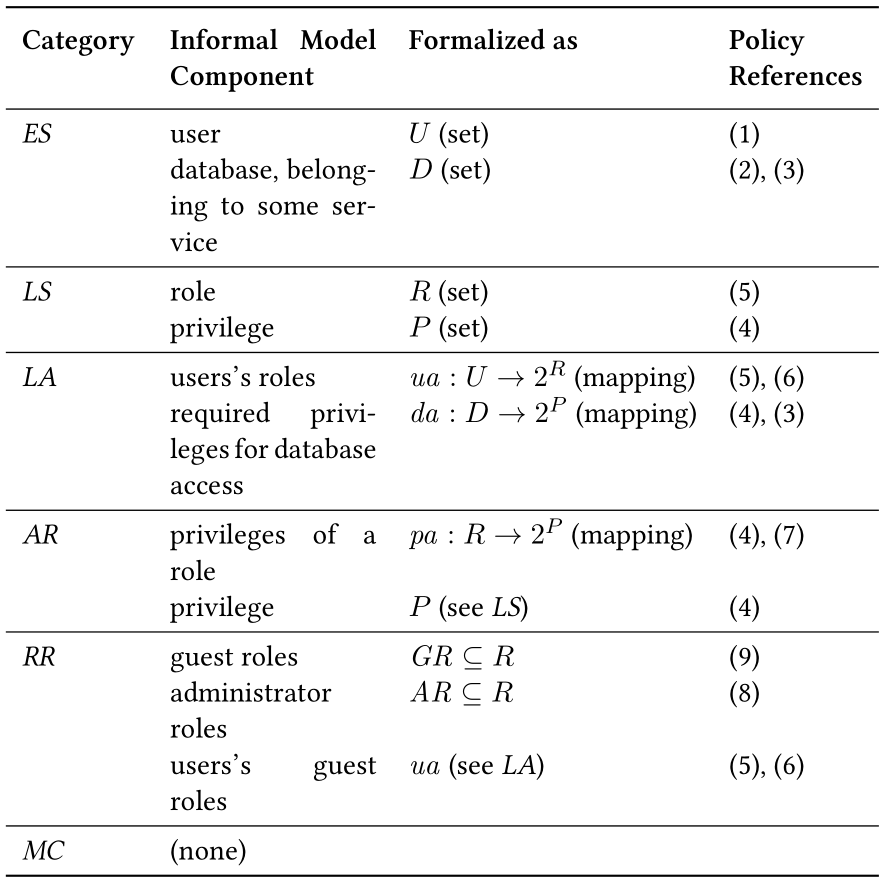
\includegraphics[width=\linewidth-3cm]{../figures/chapter2/EL_table.png}
	\caption{Result of EL-based model engineering \cite[p.77, table 4.1]{Amthor18}}
	\label{fig:EL_table}
\end{figure}

\noindent
The first column contains the EL categories.
The second column shows all given informal model components.
They are classified into the EL categories by assigning them into the corresponding row.
In the third column those model components are formalized as sets, mappings, relations, etc.
The last column refers to the corresponding informal rule of the example policy the model components originate from.

\begin{figure}[htb]
	\centering
	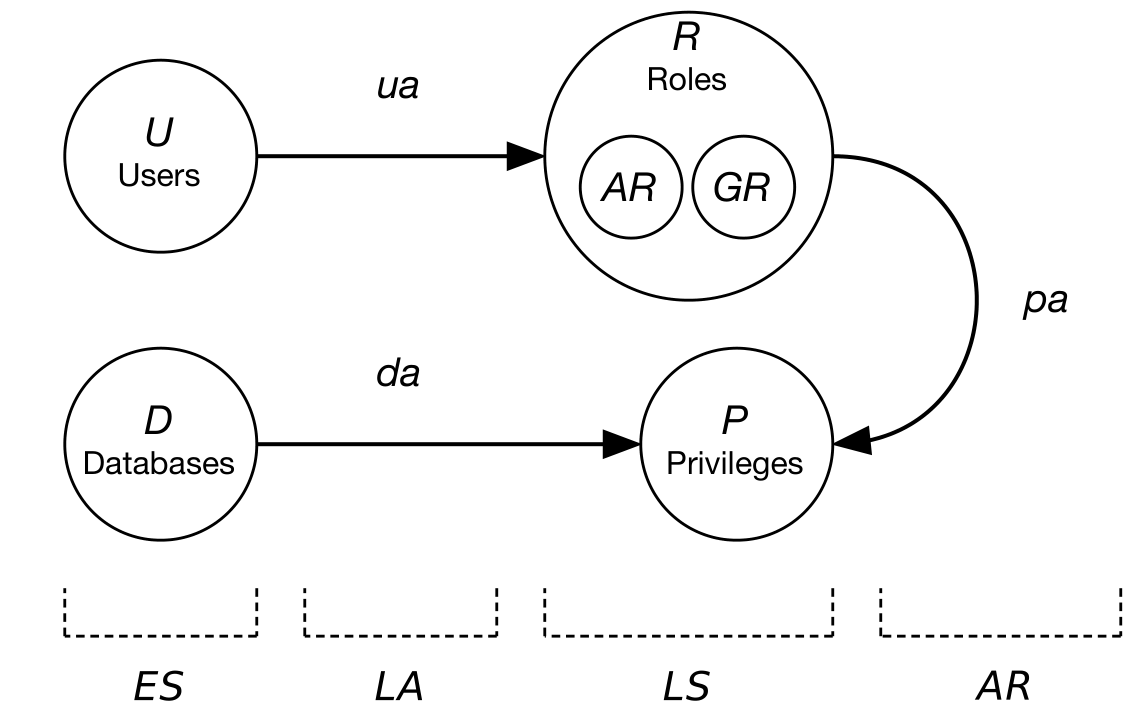
\includegraphics[width=\linewidth-6cm]{../figures/chapter2/EL_diagram.png}
	\caption{Visual summary of figure \ref{fig:EL_table} \cite[p.76, figure 4.3]{Amthor18}}
	\label{fig:EL_diagram}
\end{figure}

\cite{Amthor18} also used a graphical depiction (see figure \ref{fig:EL_diagram}) that is loosely based on the notation by \cite{Sandhu96} (see section \ref{RBAC_notation}).
In this diagram members of EL categories are visually classified by being horizontally aligned to a category space.
The category spaces are indicated with dotted lines at the bottom of the diagram.

As in the RBAC notation (see section \ref{RBAC_notation}) circles are used to depict sets.
Subsets are depicted as smaller circles inside their supersets.
Simple one-headed arrows depict mappings.
Arrows are drawn between members of \textit{ES} or \textit{LS}.
They just indicate a direction and not any properties or typing of the given relationships.
In figure \ref{fig:EL_diagram_m} there is also a double-headed arrow for depicting a relation (again analogue to the RBAC notation).

In contrast to its graphical origin -- the RBAC notation by \cite{Sandhu96} -- this notation is tailored specifically to the domain of EL.
It roughly takes the RBAC notation, simplifies it to some degree (less arrow head types, ignoring set elements) and extends it with dotted sections to indicate its EL categories.
However this notation is also imprecise and ambiguous to some extent.
This especially becomes noticeable when comparing this notation to the table form.
In chapter \ref{gsl_design} we will start off with this notation and try to identify its weaknesses to create a unambiguous and therefore more powerful notation.

\subsection{Hierarchical Entity Labeling}
\label{HEL}
To further improve scalability another level of indirection can be iteratively added to a model which already has one level of indirection (e.g. adding a role hierarchy like RBAC has).
For this additional \textit{LS} and \textit{LA} components are added to the EL categories.
In this context $m$ indicates the degree of indirection.
For $m>1$ the EL aspect is defined by \cite{Amthor18} as:

\begin{align*}
\mathcal{A}_{EL(m)} = \lbrace ES,LS_1, \dots,LS_m, LA_1, \dots, LA_m,AR,RR,MC\rbrace
\end{align*}

\noindent
Adding a role hierarchy to our example policy from above will alter $sem(LA)$ to $sem(LA_1)$ and $sem(LS)$ to $sem(LS_1)$ and will add following two assignments:

\begin{align*}
sem(LS_2) &= \lbrace R \rbrace\\
sem(LA_2) &= \lbrace RH \rbrace\\
\end{align*}

\noindent
This leads to a diagram with an additional component $RH$ and multiple sections for $LS_i$ and $LA_i$ as depicted in figure \ref{fig:EL_diagram_m}.
The category spaces at the bottom are now not the only indications for categories in this diagram.
$LA_2$ and $LS_2$ are depicted as dotted-lined rectangles within the diagram itself and frame its components $RH$ and $R$.

\begin{figure}[htb]
	\centering
	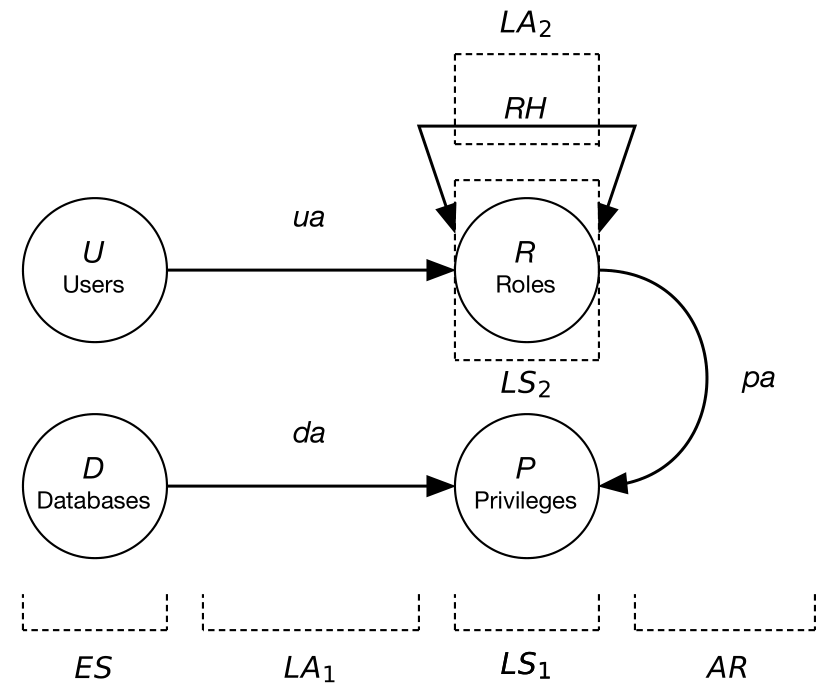
\includegraphics[width=\linewidth-6cm]{../figures/chapter2/EL_diagram_m.png}
	\caption{Visual summary with $m=2$ (not showing \textit{AR} and \textit{GR}) from \cite[p.79, figure 4.4]{Amthor18}}
	\label{fig:EL_diagram_m}
\end{figure}



\section{Graphical notation models}
\label{graphical_notations}
In this section two well-established graphical notation models are presented: UML and ER.
Due to being standard and de facto standard, they have a high relevance in the domain of graphical modeling. 
UML and ER come with reasonable concepts to illustrate structural information and semantic properties (for types of information visualization in science see section \ref{perception}).

\subsection{Unified Modeling Language}
\label{UML}
The \textit{Unified Modeling Language} (UML) is a graphical modeling language to specify, visualize, design and document software \citep{UML_OMG}.
UML became a widely used tool in software development and was standardized by The Object Management Group in 1997 and also was approved as official ISO standard in 2005 \citep{UML_ISO}.

%UML defines terms and relationships between those terms, as well as a graphical notation for those.
The current version of UML (2.5) contains 14 different types of diagrams.
Every diagram illustrates information according to one specific aspect.
UML diagrams are classified into static and dynamic types, but they can have fuzzy borders and mixed forms as well.
Static diagram types describe structural properties, dynamic diagram types behavioral properties.



\subsubsection{Components}
Components an UML diagram is build up with are classified into \textit{elements} and \textit{relationships}:

\begin{description}
\item[1) Elements]\hfill \\
Elements are the main artifacts in an UML diagram.
Graphically elements are based on closed shapes like boxes or ellipses.
They usually have a name or identifier in form of text in the center of their shape. Horizontal lines can be used to separate an element into two or more sections (see \textit{class} element). \\
Examples for elements are classes, packages, ports, etc.~(see figure \ref{fig:UML_elements}).
Elements can be closely tied to specific diagram types (e.g.~components to component diagrams).

\begin{figure}[htb]
	\centering
	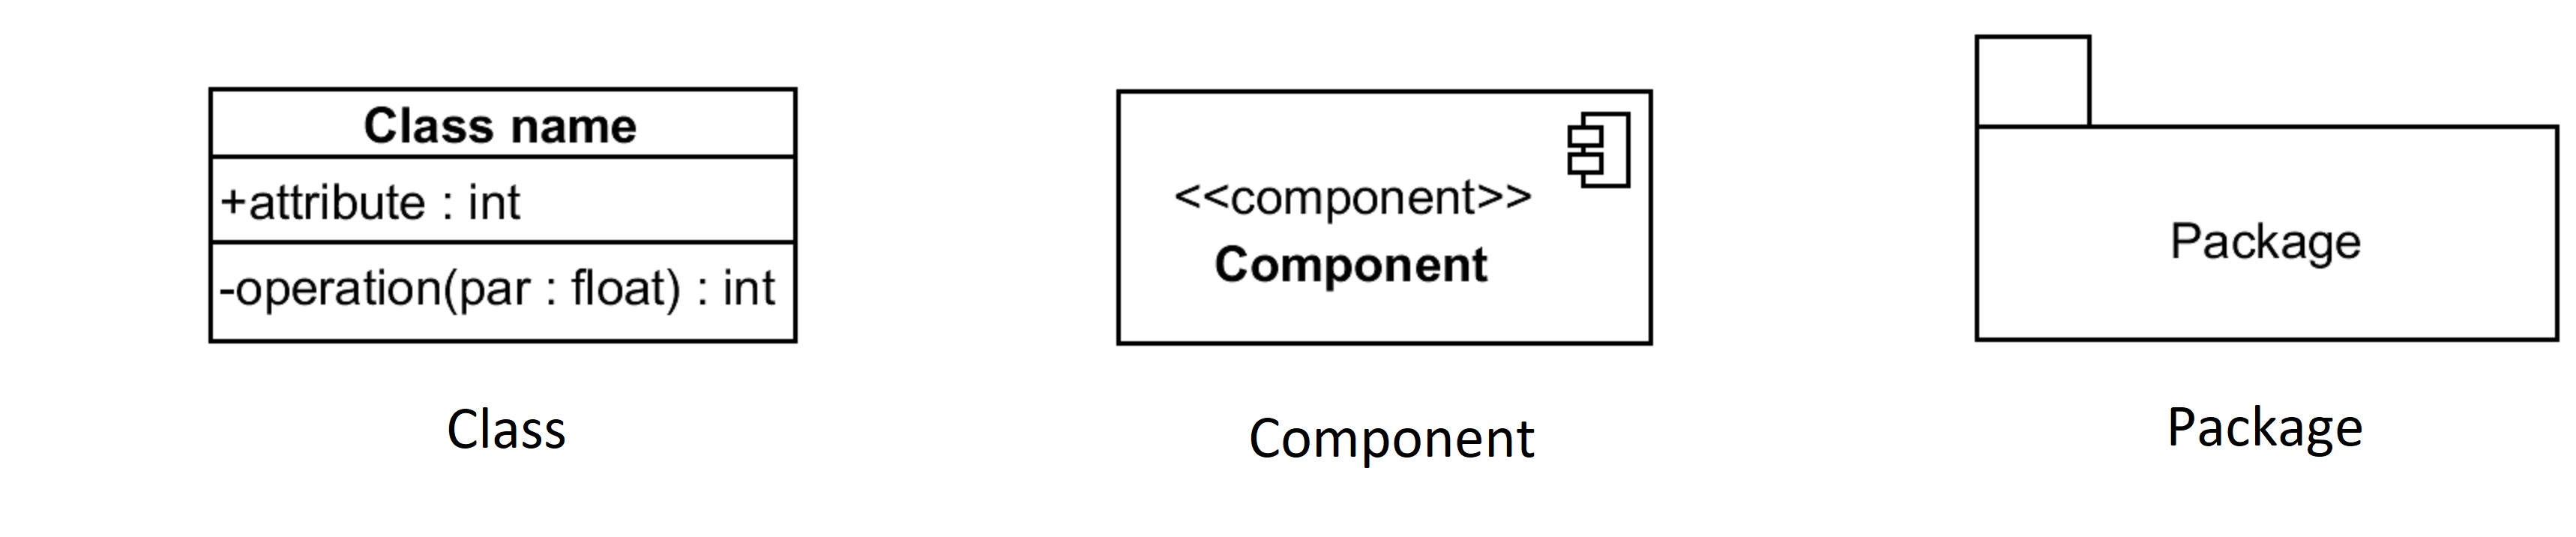
\includegraphics[width=\linewidth]{../figures/chapter2/UML_elements.png}
	\caption{Selection of UML elements}
	\label{fig:UML_elements}
\end{figure}

%\noindent 
%Some elements can have multiple forms.
%For example the class element has a simple symbolic form as well as an extended form with detailed information (see figure \ref{fig:Class}).
%With this option whole diagrams can be dynamically adjusted to a desired level of detail.
%
%\begingroup
%\leftskip10em
%\begin{figure}[htb]
%	\centering
%	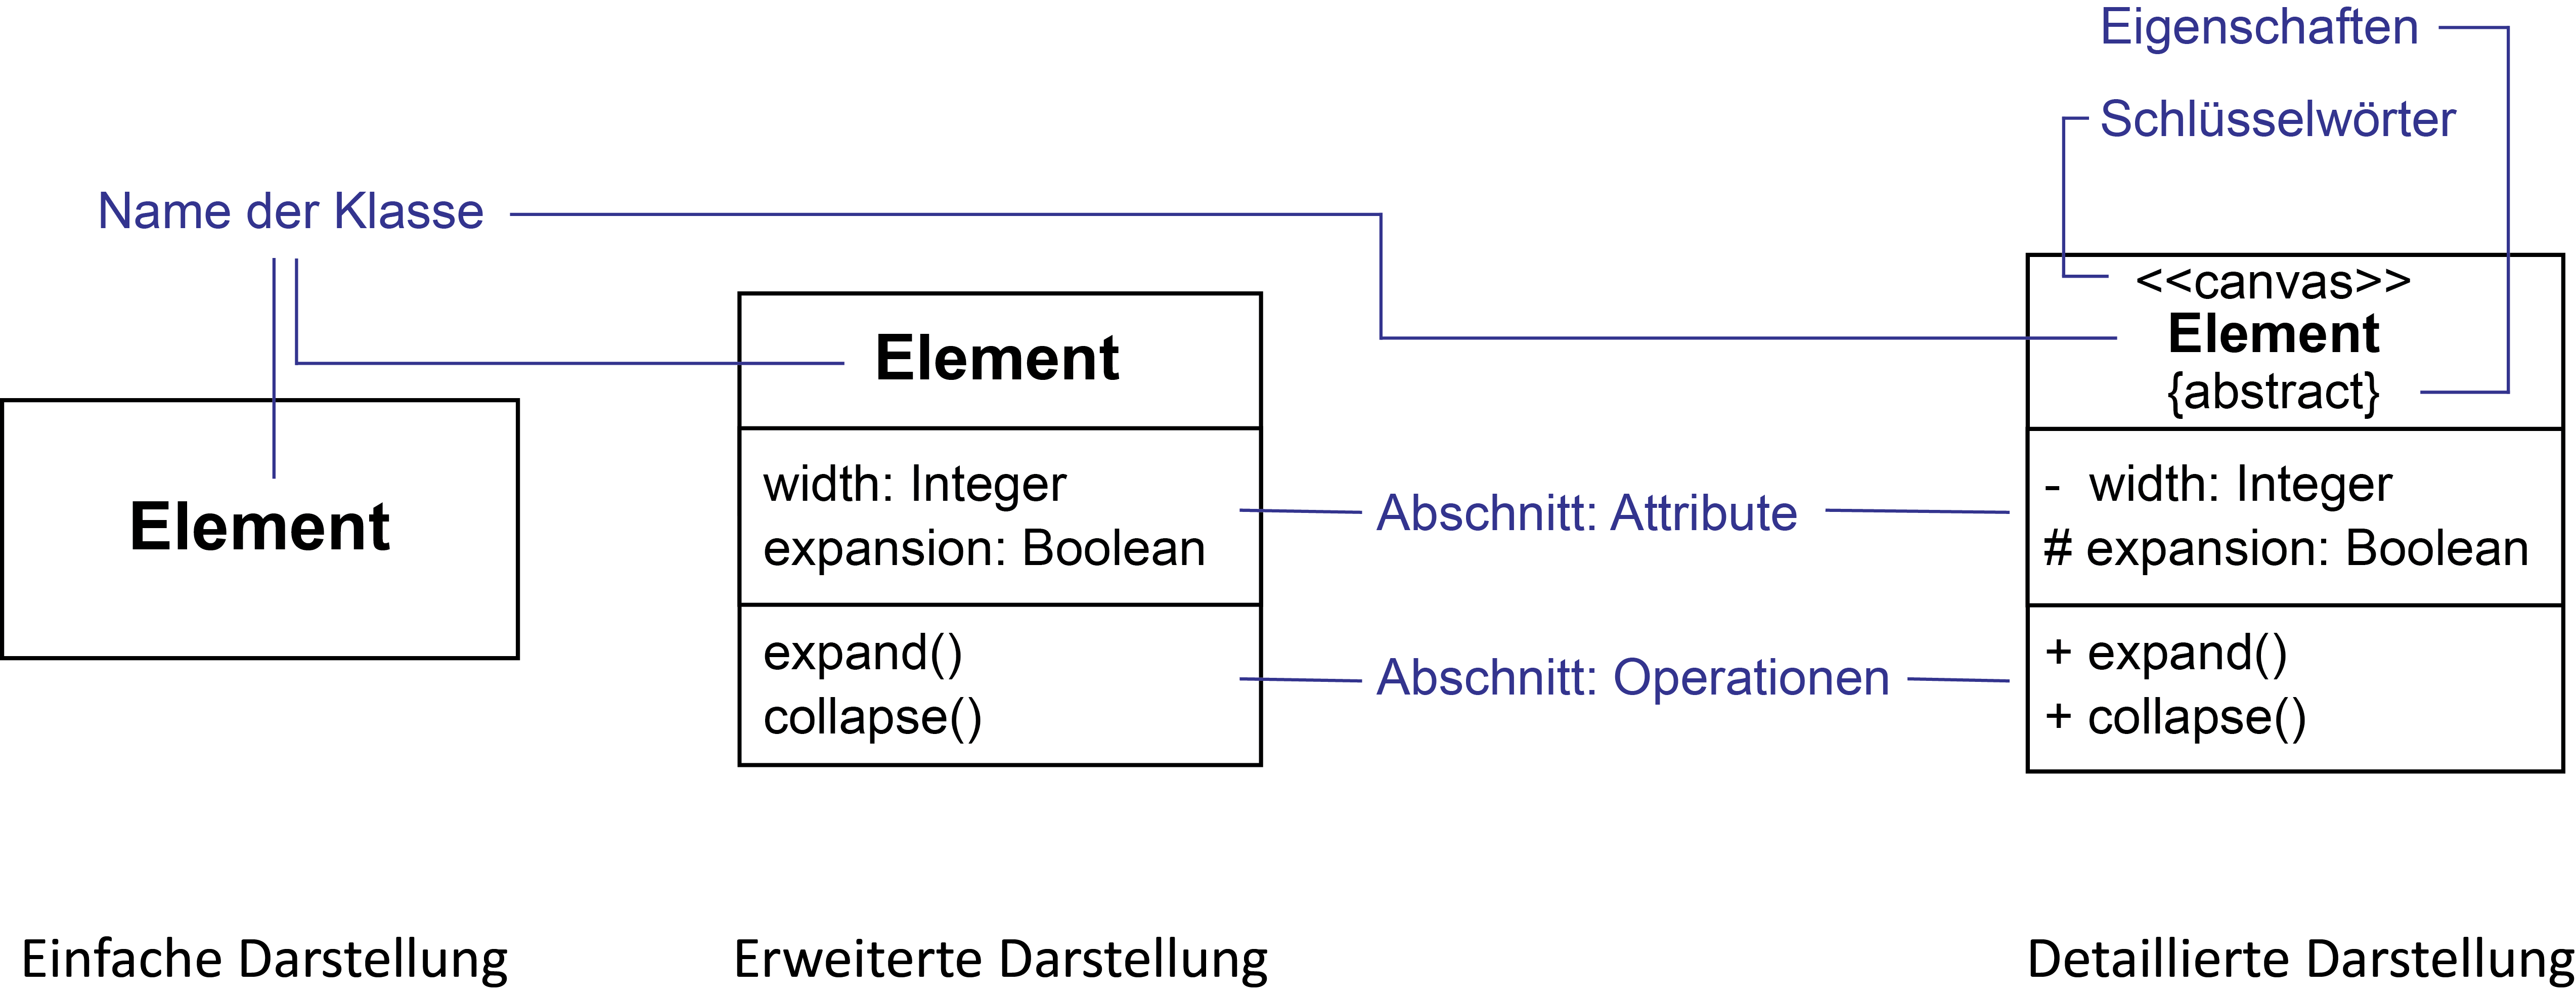
\includegraphics[width=\linewidth]{../figures/chapter2/UML_Klassen2.png}
%	\caption{Class diagrams with different level of detail}
%	\label{fig:Class}
%\end{figure}
%\par
%\endgroup

\item[2) Relationships]\hfill \\
Relationships can connect two or more elements.
Graphically relationships are lines.
Optionally they can have a shape at one end to indicate a direction.
They can vary in form by having differently drawn lines (solid, dotted) or shaped arrow heads.
They can have several angles (preferable $90^{\circ}$ or $45^{\circ}$) to run on a clearly laid out path.
Lines do not collide if possible. \\
Examples: Dependency, generalization, include (see figure \ref{fig:UML_relationships})

\begin{figure}[htb]
	\centering
	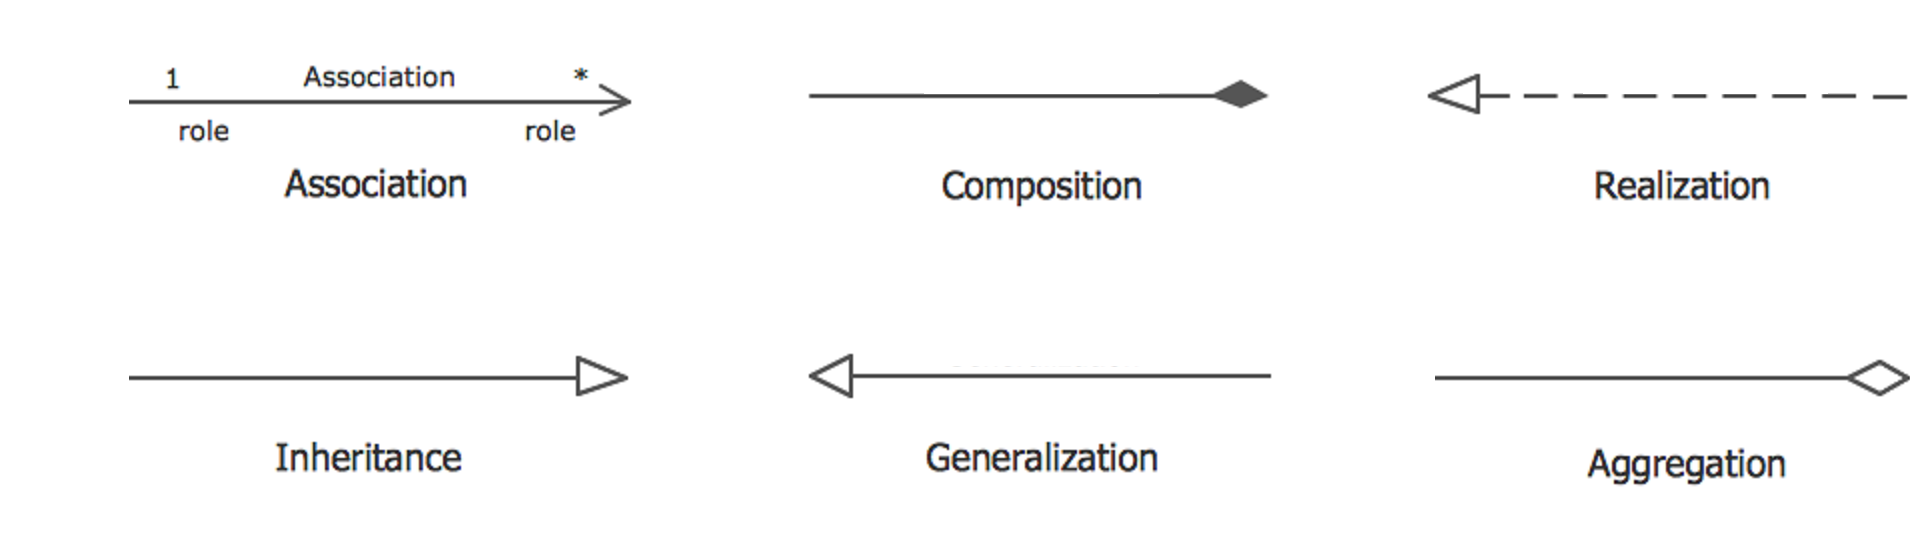
\includegraphics[width=\linewidth]{../figures/chapter2/UML_relationships.png}
	\caption{Selection of UML relationships}
	\label{fig:UML_relationships}
\end{figure}
\end{description}



\subsubsection{Additional annotations}
UML has symbols and textual identifiers to visualize certain properties.
With \textit{multiplicities} an element can be constrained regarding its number in context of an relationship.
The notation is placed at the connection point of class and relationship component.
In almost all cases it is depicted as integer number (0 or 1) or * to indicate a boundless interval.

Furthermore it is worth mentioning that UML does not use any color for its diagrams.
This makes it compatible, easy and fast for hand-drawing.
Coloring remains a not officially specified option to highlight certain parts of a diagram, e.g. to set a focus without being in conflict with any already colorized sections of the model.


\subsection{Entity-Relationship model}
\label{ER}
The entity-relationship model (ER) is a model to describe classified objects (entities) and how they are interrelated.
It was developed to illustrate information in databases on a conceptual level and became a popular tool for requirement analysis in this domain.
In contrast to UML (see section \ref{UML}) ER only has one type of diagram: The Entity-Relationship diagram (ERD).
Also unlike UML ER is not an officially specified standard.
ER has different notation variants (Chen, Bachman, etc.), which will be depicted in section \ref{ERD_notations}.
Figure \ref{fig:ERD_minimal_example} shows an example of an ERD.


\begin{figure}[htb]
	\centering
	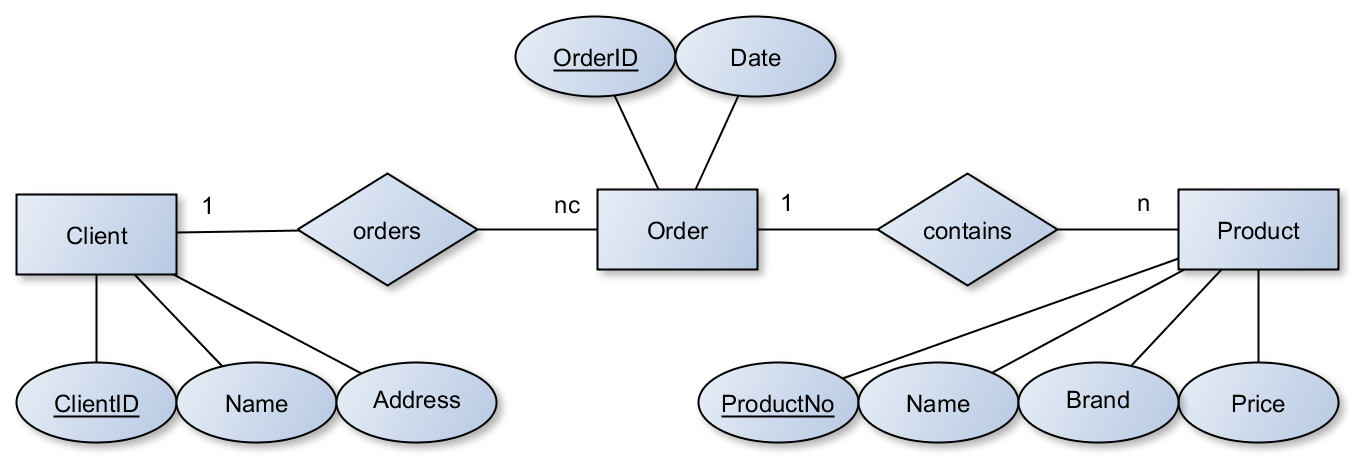
\includegraphics[width=\linewidth]{../figures/chapter2/ERD_minimal_example.png}
	\caption{ERD example}
	\label{fig:ERD_minimal_example}
\end{figure}

\subsubsection{Components}
ERDs are build up with the following components \citep{Kleuker11}:

\begin{description}
\item[1) Entity type]\hfill \\
The most important artifact of ER is probably the entity.
It represents an individual and unambiguously identifiable object.
An entity is characterized by its properties.
An \textit{entity type} is a template for entities that summarizes all their attributes.
Entities can be interpreted as instances of an entity type with concrete values.
Graphically an entity type is a simple rectangle with its name in its center.

\begin{figure}[htb]
	\centering
	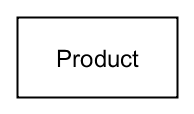
\includegraphics[scale=0.4]{../figures/chapter2/ERD_entity.png}
	\caption{Entity object of an ERD}
	\label{fig:ERD_entity}
\end{figure}

\item[2) Relationships]\hfill \\
Relationships can connect two or more entities and describe how they are interrelated.
In contrast to UML (see \ref{UML}) relationship is not represented with a simple lines, but with a rhombus with the relationship name in its center.
This rhombus is then connected to two or more entities with simple lines.
These lines may have symbols at their end to indicate properties of the connected entities in context of the relationship.

\begin{figure}[htb]
	\centering
	
\includegraphics[scale=0.4]{../figures/chapter2/ERD_relationship.png}
	\caption{Relationship object of an ERD}
	\label{fig:ERD_relationship}
\end{figure}

\item[3) Attributes]\hfill \\
Attributes are properties of entites or relationships.
Graphically an attribute is a single ellipse with its name in its center.
It is connected to an entity or to a relationship with the help of a simple line.

\begin{figure}[htb]
	\centering
	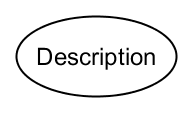
\includegraphics[scale=0.4]{../figures/chapter2/ERD_attribute.png}
	\caption{Attribute object of an ERD}
	\label{fig:ERD_}
\end{figure}
\end{description}

\subsubsection{Additional annotations}
To specify the amount of entities in context of a relationship the following indicators for \textit{cardinalities} are used:

\begin{itemize}
\setlength\itemsep{0em}
\item \textbf{1} to indicate a relationship to exactly one entity.
\item \textbf{c} to indicate a relationship to no or one entities.
\item \textbf{n} to indicate a relationship to one or multiple entities.
\item \textbf{nc} to indicate a relationship to no, one or multiple entities.
\end{itemize}

\noindent
%Cardinalities can be upper case (N) or lower case (n) with no semantic difference.
A relationship can be read in two directions.
For example the \textit{orders}-relationship in figure \ref{fig:ERD_minimal_example}:

\begin{itemize}
\setlength\itemsep{0em}
\item An order is connected to exactly one client (left-to-right).
\item A client is connceted to no, one or multiple orders (right-to-left).
\end{itemize}

\noindent
An entity type needs to have a \textit{primary key} defined in order to have its elements unambiguously identifiable.
The primary key is an attribute or a combination of attributes of the entity type and has to be unique among all other attribute values.
A primary key attribute is graphically indicated with an underlined name (see \textit{ClientID} in figure \ref{fig:ERD_minimal_example}).

%Besides this basic system, ERDs can indicate some additional information.
%For example besides those elements described above, there are variants of them with a double frame line to indicate a \textit{weak} property (no primary key, dependent to parent elements) or a dashed frame line to indicate a \textit{multivalued} property.
%In context of this work those will not be relevant.



\subsubsection{ERD Notation Variants}
\label{ERD_notations}
As already mentioned ER is not standardized and has different notation variants.
These variants only differ in the depiction of their relationships (see figure \ref{fig:ERD_notations}).

\begin{figure}[htb]
	\centering
	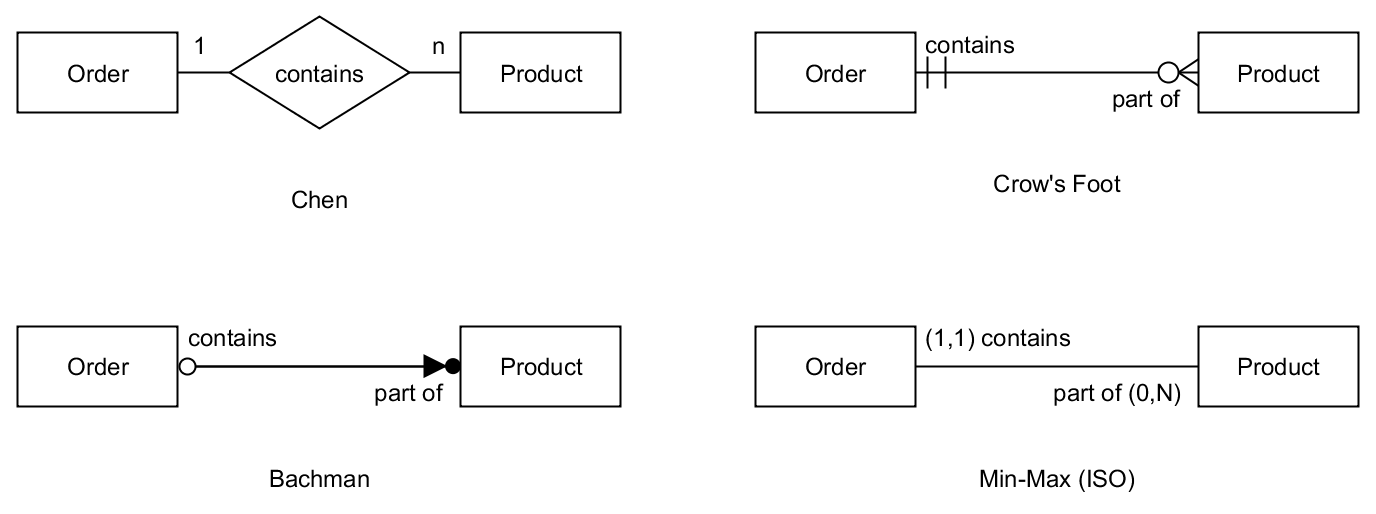
\includegraphics[width=\linewidth+0.3cm]{../figures/chapter2/ERD_notations.png}
	\caption{ERD notation variants}
	\label{fig:ERD_notations}
\end{figure}

%\noindent
% ERD as UML
Notable is also that an ER model can be visualized with the help of UML.
When entity types are treated as classes, entities as objects, relationships as associations, attributes as instance variables and cardinalities as multiplicities an UML \textit{class diagram} can be used to build up a diagram that is similar to an ERD.

\begin{figure}[htb]
	\centering
	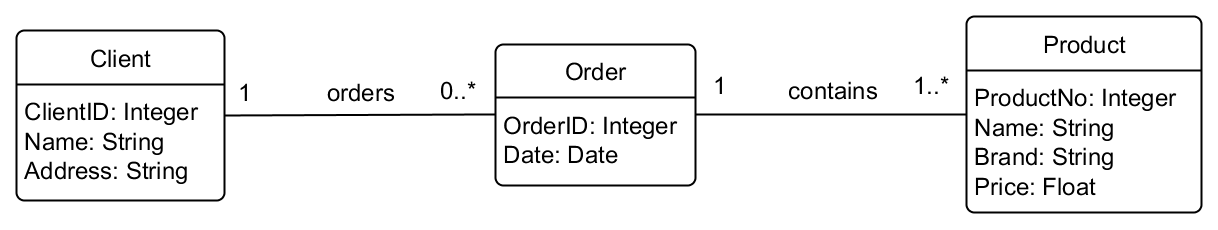
\includegraphics[width=\linewidth+0.2cm]{../figures/chapter2/ERD_as_UML.png}
	\caption{ERD modeled as UML class diagram}
	\label{fig:ERD_as_UML}
\end{figure}

%\noindent
%As seen in figure \ref{fig:ERD_as_UML} the diagram visually differs from the diagram in figure \ref{fig:ERD_minimal_example}, but can depict the information even more compact.
%However, there is no common way for indicating an entity type's primary key in UML (the UML extension concept of \textit{stereotypes} can be used for this).



\section{Perception}
\label{perception}
This section is about the human visual perception.
Its content will act as fundamental basis for designing a graphical specification language in chapter \ref{gsl_design} as well as for designing an editor's graphical user interface in chapter \ref{editor_design}.

In science there are two types of visualizing information:
One is to present absolute or relative primitive values (tables, bar graphs, pie charts) and one to depict structural information and semantic properties (specialized graphical systems like the class diagram of UML or the Chen notation of ERD).
Designing a new system of the latter should consider design guidelines and rules of best practice to visually support working with it.
One of these are gestalt laws.

\subsection{Gestalt Laws}
\label{gestalt_laws}
Gestalt laws (from German \textit{Gestalt}: shape, form) are derived from findings in the human perception of visual content.
They describe phenomena of how we perceive and evaluate objects and groups of objects in context to each other intuitively.

These laws apply in particular when we look at graphical user interfaces (\textit{GUI}), graphs or diagrams.
They can describe how and why we look at certain aspects first or find some aspect more easy or hard to understand than another.
Considering gestalt laws while designing any graphical content can improve its perception quality and therefore also the handling for its readers or users.

Given that there is a large number of various gestalt laws, the following list (based on \citep{Goeckel01a}, \citep{Heinecke04a} and \citep{Sternberg}) describes some of them that are relevant for the task of designing a graphical specification language in chapter \ref{gsl_design}:

\begin{description}
\item[1) Law of Prägnanz]\hfill \\
The Law of Prägnanz (German for \textit{pithiness}) is the fundamental principle of gestalt laws.
It says that humans tend to order inputs of their senses in the best possible way (simple, regular, symmetrical).
This results in phenomena like completing incomplete forms or favoring closed objects or treating groups of objects as units.

\item[2) Law of Proximity]\hfill \\
Objects that are closer together are not associated individually but as groups.
Smart utilizing this law offers opportunities to design visually separated sections without the help of any lines or boxes.

\item[3) Law of Similarity]\hfill \\
Homogeneously depicted objects are associated as belonging together, although they may not be in close range to each other.
This effect can be induced by \textit{Gestalt factors} like shape, color, brightness, size, orientation or rotation.
%This law allows classifying or logically grouping multiple spatially distributed objects.

\item[4) Law of Good Gestalt]\hfill \\
While looking at complex structures of objects, details are ignored and objects will always be perceived in the most simple, regular and symmetric pattern they will form.

\item[5) Law of Good Continuation]\hfill \\
Two overlapping objects are often perceived as uninterrupted.
This law allows straight lines to intersect without any confusion.
\end{description}



\subsection{Human Optical Perception}
\label{human_optical_perception}
\textit{Semiosis} is the science of signs.
It deals with analyzing signs and how they transport information \citep{Zeckzer14a}.
Semiosis differentiates between \textit{sensory symbols} and \textit{abstract symbols}.
Sensory symbols are based on biologically preset perception processes and can be recognized without any additional information (e.g.~the shape of a human body).
Abstract symbols can be chosen freely and have to be learned, because they have no relation to its reference (e.g.~the mathematical sign for infinity $\infty$).
Software applications use sensory symbols to make its functions independent from text (and therefore a specific language).
Besides sensory symbols also abstract symbols have established for common actions (e.g.~\textbf{+} to add, \textbf{-} to remove, \textbf{ \underline{ }} to minimize, \textbf{$\times$} to close, etc.)

\cite{Zeckzer14a} describes that humans are able to hold 3 to 7 elements in their visual buffer inside their short term memory.
This buffer size limits our processing capacity and visual awareness.
Handling more than this number of symbols will result in understanding a graphical system more ineffectively.

According to \cite{Ware04a} optical stimuli are perceived and processed in three consecutive steps with differently set priorities depending on their content:

\begin{description}
\item[1) Parallel processing to extract low-level characteristics]\hfill \\
In this first step inputs are processed in parallel by millions of neurons in high speed.
The inputs are then evaluated regarding their orientation, movement and overall color impression.

\item[2) Perception of pattern and structures]\hfill \\
In this second step the picture gets separated into regions.
Simple structures like contours, colors and textures get recognized.
Object recognition begins.

\item[3) Sequential target-oriented processing]\hfill \\
In this last step single recognized objects get selected and stored in the short term memory.
There they are ready for further processing, e.g.~applying of knowledge or emotions.
\end{description}



\section{GUI Design}
\label{gui_design}
The \textit{graphical user interface} (GUI) is a well-established interface type that allows interactions between human and machine on a graphical level.
It presents visual content to its users and offers functions to operate with the help of symbols and control elements.
GUIs were developed, because text-based \textit{command line interfaces} (CLI) need a higher degree of memorization and familiarity for operation and navigation and therefore new users in particular find operating a CLI more difficult than a GUI \citep{CLI}.
Unfortunately GUI design often lacks ease of use, due to its design being tied too strictly to the work flow of experts \citep{Reckling14}.

There are some best practices to stick to when it comes to design a \textit{good} GUI.
One of them is to reuse already established methods and approaches like \textit{user interface pattern}.
Another one is to evaluate whether a design concept follows \textit{usability} rules.



\subsection{Usability}
\label{usability}
\cite{Shackel91a} defines usability as following:

\begin{xdefinition}[Usability] 
Usability is the capability to be used by humans easily and effectively, while
\begin{itemize}
\item \textit{easily} means ``to a specified level of subjective assessment'' and
\item \textit{effectively} means ``to a specified level of (human) performance''
\end{itemize}
\label{definition:usability}
\end{xdefinition}

\noindent
Usability can be classified into \textit{interaction design} and \textit{interface design}.
The former describes \textit{how} a system reactions to user interactions, the latter \textit{with what} a system visualizes interaction options \citep{Reckling14}.

\cite{Tidwell11} describes several principles essential for achieving a high usability.
These principles can be applied in form of non-functional requirements in the process of designing a new GUI.
The following list describes the first 6 of those principles:

\begin{description}
\item[1) Safe Exploration]\hfill \\
A user should always be able to safely explore the interface.
This includes undoing every operation he performs in particular.
%For this a software has to be designed as \textit{non-destructive} as possible.

\item[2) Instant Gratification]\hfill \\
A user should always instantly get feedback about operations he just performed.
This can be the direct result of his operation (e.g.~opening a window) or a visual hint, that an operation was executed as desired (e.g.~coloring an activated button).

\item[3) Satisfiscing]\hfill \\
\textit{Satisfiscing} (\textit{satisfying} and \textit{sufficing}) is the phenomenon that a user tends to scan all options just roughly and to use trial-and-error before finding the perfectly matching tool for a certain task.
He tends to be fine with solutions that are \textit{good enough} and not the best possible.
This means that the user should be supported to find the right tools when he needs them.
%For this symbols and texts have to be short, simple and easy to understand.
Elements and symbols already known should be reused when possible.
Also to ensure a correct order of operations or work flow (if necessary at all, see point 6 of this list) the user should be guided appropriately (e.g.~\textit{drag here}).

\item[4) Changes in Midstream]\hfill \\
A user should always be able to interfere with running operations to always have the control (e.g. a time consuming operation indicated with a progress bar together with a cancel button underneath).

%\item[5) Deferred Choices]\hfill \\
%A user should always be able to defer choices that are not mandatory and answer just the minimal set of questions that are necessary to progress at a certain point.
%Of course, besides this, the system has to offer a way for the user to come back to answer the skipped questions later.

\item[5) Incremental Construction]\hfill \\
Builder-style software like editors need to support \textit{incremental construction}.
This means that the user is free to choose on which particular part he wants to works.
A user should always be free to stop working on one part and instantly jump to another part to continue working there.
When this \textit{incremental construction} is achieved to a high degree, this can induce a state of flow in the user, which leads to an increased working performance and satisfaction.
\end{description}


\subsection{Interaction Design Patterns}
\label{design_patterns}
A GUI has to be designed a way it can be operated mostly intuitively.
This means that a user should find his way without knowing a new application.
This can be achieved by reusing graphical control elements and functions that are already well-established and known from working with other software's GUI.
These elements can be recognized by their similar visual appearance and will always work in a similar known way.
These elements are called \textit{interaction design patterns}.

An interaction design pattern is defined by \cite{Folmer} as a general repeatable solution to a commonly-occurring usability problem in \textit{interface} or \textit{interaction design}.
Interaction design pattern can be graphical elements like buttons, menus or scroll bars as well as control functions like drag and drop, swipe gestures or context-menu by clicking the mouse button.

Whenever these patterns fit, they should be applied.
Reinventing interaction design is not only very time consuming, but actually even counterproductive concerning usability due to users will get discouraged by being confronted with new unknown mechanisms (see section \ref{usability} \textit{satisfiscing}).



\cleardoublepage
\chapter{Design: Graphical Specification Language}
\label{gsl_design}


\section{Concept}
\label{gsl_concept}
approach, basic ideas, adoptions from literature

Due to being highly tailored to one specific domain these visualizations are impractical for direct reuse in another domain.
Generally a new application will also require a newly designed graphical system.
In reality certain components and ideas already established in other well-known or related systems are getting (partly) reused and adapted accordingly.
A newly designed graphical system should be designed in a way its components are not ambiguously compared to similar systems from related domains to avoid misunderstanding.



%This law allows classifying or logically grouping multiple spatially distributed objects.




\section{Elements}
\label{gsl_elements}


\section{Relationships}
\label{gsl_relationships}


\section{Structure}
\label{gsl_structure}


\section{Visualization on a Higher Level of Abstraction}
\label{higher_abstraction_level}




\cleardoublepage
\chapter{Design: Editor GUI}
\label{editor_design}


\section{Structure}
\label{editor_structure}


\section{Sections}
\label{editor_sections}




\cleardoublepage
\chapter{Implementation}
\label{implementation}
	
	
\section{Implementation Base}
\label{implementation_base}
Qt, MVC

\section{Structure}
\label{implementation_structure}
	
	
\section{GUI sections}
\label{implementation_sections}




\cleardoublepage
\chapter{Evaluation}
\label{evaluation}


\section{Graphical Specification Language}
\label{evaluation_gsl}


\section{Editor}
\label{evaluation_editor}


\cleardoublepage
\chapter{Conclusion}
\label{conclusion}
\blindtext



\cleardoublepage
\chapter{Summary}
\label{summary}
\blindtext



% Anhang
%\cleardoublepage
%\tocentry{Anhang}
%\renewcommand{\thesection}{\Alph{section}}
%\markboth{Anhang}{}
%\chapter*{Anhang}
%\section{Kapitel 1}
%\section{Kapitel 2}
%\label{appendix}




% Literaturverzeichnis
\cleardoublepage
\DeclareRobustCommand{\citeext}[1]{\citeauthor{#1}~\cite{#1}}
\bibliographystyle{plainnat}

\bibliography{other/db}

\tocentry{Bibliography}





\end{document}